%!TEX root = Python.tex

\chapter{Introducción}

\lettrine[lines=5]{A}{} partir del curso 2018/2019, la asignatura de Autómatas y Lenguajes Formales comienza a emplear Python en las prácticas de programación. Emplear este lenguaje conlleva algunas ventajas con respecto a su predecesor, Java. En primer lugar, el lenguaje Python se concibió para que fuese fácil de aprender. En las primeras semanas del curso se impartirán seminarios sobre este lenguaje que darán las bases para desarrollar aplicaciones de validación de cadenas con autómatas finitos y expresiones regulares, y de traducción entre formatos de ficheros. Además, Python es un lenguaje en continua expansión, cada vez más usado en sectores con una fuerte proyección de futuro, como el análisis de datos, el cálculo científico y la bioinformática. Creemos que el hecho de usar uno de los lenguajes más populares en la actualidad puede dar una mayor motivación para abordar las prácticas de la asignatura.

Es necesario realizar una \emph{advertencia} antes de seguir: estos apuntes no son un manual del lenguaje Python. Únicamente pretenden recoger lo que es necesario para abordar los problemas tratados en la asignatura. Además, están enfocados a alumnos que tienen cierto conocimiento del lenguaje C, ya que en numerosas ocasiones se compara la forma de realizar algo en este lenguaje y en Python. Para un estudio más amplio de Python, se recomienda la consulta de las referencias bibliográficas que aparecen al final de estos apuntes.

\section{Breve historia de Python}

El lenguaje Python fue concebido inicialmente por el informático holandés Guido Van Rossum, cuando trabajaba en el \emph{Centrum Wiskunde \& Informatica}\footnote{Centro para las Matemáticas y la Ciencia de la Computación (\url{http://www.cwi.nl}).} (CWI) de Ámsterdam hacia finales de los ochenta. Van Rossum formaba parte del equipo dedicado al desarrollo del sistema operativo distribuido \emph{Amoeba} (proyecto liderado por Andrew Tanenbaum), y su objetivo al crear Python era proporcionar un lenguaje de programación que pudiese cubrir el hueco que existía en Amoeba entre el lenguaje C y el shell del sistema. Hacía falta un lenguaje de alto nivel con mayor potencia expresiva que el shell pero sin las dificultades de C, que en Amoeba tenía un interfaz de programación con el sistema bastante complicado. 

Según el propio Van Rossum\footnote{En el blog de Guido Van Rossum sobre la historia de Python (http://python-history.blogspot.com), se puede leer lo siguiente: \emph{I picked the first thing that came to mind, which happened to be Monthy Python’s Flying Circus, one of my favorite comedy troupes. The reference felt suitably irreverent for what was essentially a “skunkworks project”. The word “Python” was also catchy, a bit edgy, and at the same time, it fit in the tradition of naming languages after famous people, like Pascal, Ada, and Eiffel. The Monty Python team may not be famous for their advancement of science or technology, but they are certainly a geek favorite. It also fit in with a tradition in the CWI Amoeba group to name programs after TV shows.}}, el nombre del lenguaje es un homenaje a los cómicos ingleses Monty Python. Existen lenguajes cuyos nombres proceden de personajes famosos, como Pascal, Ada o Eiffel. Python sería, salvando las distancias, una continuación de esta tradición. 

\begin{figure}
\captionsetup[subfigure]{labelformat=empty}
\begin{subfigure}{0.48\textwidth}
\includegraphics[width=\linewidth]{imagenes/Guido-van-Rossum}
\caption{Guido Van Rossum} \label{fig:guido-van-rossum}
\end{subfigure}
\hspace*{\fill} 
\begin{subfigure}{0.48\textwidth}
\includegraphics[width=\linewidth]{imagenes/Monty-Python}
\caption{Monty Python} \label{fig:monty-python}
\end{subfigure}
\caption{Personajes relevantes en el origen de Python}
\end{figure}

Una de las fuentes de inspiración de Van Rossum para la concepción de Python fue el lenguaje \emph{ABC}, también desarrollado en el CWI de Ámsterdam, que pretendía ser un sustituto del lenguaje \emph{BASIC} (aparecido hacia los sesenta) para la enseñanza de la programación. Python tiene una sintaxis en la que la sencillez es un principio esencial para atraer a programadores noveles, pero también asume algunas notaciones sintácticas propias de lenguajes con mucha implantación, como C, para que los programadores experimentados puedan usar Python con facilidad.

La primera versión pública de Python se presenta en 1991. El año 1996, Van Rossum continúa desarrollando el lenguaje con un equipo de colaboradores en el \emph{Corporation for National Research Institute} (CNRI) en Reston, Virginia (EE.UU.), una organización sin ánimo de lucro cuyo objetivo es la promoción de las tecnologías de la información. En colaboración con la agencia estatal estadounidense \emph{Defense Advanced Research Projects Agency} (DARPA), el año 1999 se inicia un proyecto para estudiar la aplicación de Python a la enseñanza de la programación. En el año 2001 se creó la \emph{Python Software Foundation} (PSF)\footnote{Web de la fundación: \url{https://www.python.org/psf-landing/}.}, siguiendo el modelo de la fundación Apache\footnote{Fundación sin ánimo de lucro dedicada al desarrollo de aplicaciones gratuitas, empezando por el famoso servidor HTTP: \url{https://www.apache.org/}.}, y se lanzó la versión 2.1 del lenguaje que contaba con una licencia compatible con la \emph{General Public Licence} de GNU. De 2005 a 2012 Van Rossum pasa a trabajar en Google, y de 2013 a la actualidad en Dropbox, potenciando a través de estas compañías la divulgación y el uso del lenguaje Python.

Van Rossum ha sido el \emph{Benevolent Dictator for Life} (BDFL)\footnote{Dictador benevolente vitalicio.} en la comunidad de desarrolladores de Python, es decir, ha asumido la responsabilidad de tomar las decisiones finales sobre la evolución del lenguaje. Su \emph{benevolente dictadura} se ha caracterizado por una actitud conservadora, admitiendo pocos cambios al lenguaje entre versiones sucesivas. Sin embargo, no han sido nada \emph{benevolentes} las fuertes críticas que ha recibido por adoptar esta postura, hasta el punto de que, el 12 de julio de 2018, con un mensaje enviado a la lista de python-committers\footnote{En \url{https://www.mail-archive.com/python-committers@python.org/msg05628.html} se puede leer el mensaje de retirada de Guido Van Rossum. La revolución en la comunidad de Python se ha desencadenado a raíz de una acalorada discusión en torno a permitir o no el uso de asignaciones en expresiones. Se puede consultar en el Python Enhancement Proposal (PEP) 572: \url{https://www.python.org/dev/peps/pep-0572/}. Y es que, por lo que parece, la sintaxis de los lenguajes de programación desata pasiones.}, anunció su completa retirada de la toma de decisiones sobre la evolución del lenguaje. No ha nombrado a ningún sucesor, de modo que todo apunta a que se va a formar un grupo de expertos entre los desarrolladores de Python más destacados, que adoptarán las decisiones estratégicas por votación.


\section{Características principales}

Python es un lenguaje de programación cuyo uso combina un compilador y un intérprete, de forma muy similar a Java. El código de los ficheros fuente de Python, con extensión \texttt{.py}, pasa en primer lugar por un compilador, que traduce el programa desde el lenguaje Python a una versión equivalente en un lenguaje de bajo nivel, el llamado \emph{bytecode} de Python (un ensamblador de una máquina virtual). El compilador genera un fichero con extensión \texttt{.pyc} con el mismo nombre que el fichero fuente, compilando sólo los ficheros que han sido modificados.

Una vez que están todos los ficheros fuente del programa compilados, se lanza el intérprete de Python para ejecutar el programa. El intérprete tiene una concepción similar a la de la máquina virtual de Java. Carga y ejecuta los bytecodes, permitiendo que cualquier programa Python se ejecute en cualquier sistema para el cual exista un intérprete. Esto facilita la portabilidad del código Python. Tanto el compilador de referencia (\texttt{CPython}) como el intérprete de Python están escritos en el lenguaje C, garantizando de esta forma una ejecución rápida de ambos.

Aunque no es habitual en el desarrollo de aplicaciones, se puede usar el intérprete de Python interactivamente desde una consola que permite ejecutar directamente operaciones del lenguaje. Este modo de uso de Python sería equivalente al de un shell del sistema operativo, y podría emplearse para ejecutar secuencias de comandos de un solo uso. También podría permitir hacer pequeñas pruebas de código antes de integrarlo en un fichero \texttt{.py}.

Python permite desarrollar aplicaciones usando varios paradigmas de programación. El lenguaje es orientado a objetos, pero se puede usar en gran medida como lenguaje imperativo. Además, es un lenguaje dinámicamente tipado. Esto significa que no es necesario declarar las variables antes de su uso, y que a una misma variable se le pueden asignar valores de tipos de dato distintos a lo largo de la ejecución del programa. La verificación del uso correcto de los tipos en cada operación que use una variable se realiza en tiempo de ejecución.

Otra característica de Python es el manejo autómatico de la memoria. El programador no debe preocuparse de llamar a funciones que reservan o liberan memoria, evitando el manejo de punteros como en C. Además, Python incluye una librería estándar que permite realizar operaciones de gran utilidad: validación y búsqueda de cadenas con expresiones regulares, consultas sobre ficheros XML, programación de aplicaciones que usan protocolos de red como HTTP, y un largo etcétera. Por esta razón, Python es una opción muy interesante para implementar prototipos de aplicaciones de forma rápida.


\section{Entorno de desarrollo}

En esta sección se indican los pasos necesarios para disponer de una versión actualizada del compilador e intérprete de Python, integrada en la herramienta de desarrollo Eclipse, con el fin de disponer de un entorno de desarrollo similar al que está instalado en los laboratorios de la FIUM.

\subsection{Instalación de Python}\label{sec:instalacion}

En primer lugar, es necesario descargar e instalar la última versión de Python 3 en nuestro equipo. En el momento de escribir este manual, está disponible la versión 3.7.0\footnote{Resultar curioso que exista una versión 2.7.15 también reciente. Esto es así porque, en realidad, hay dos ramas de desarrollo de Python, pero nosotros emplearemos la versión 3.7.0.}.

En función del sistema que estemos empleando, tenemos dos opciones para hacer la instalación. Si usamos Windows o Mac OS X, podemos descargar el instalador que necesitemos, y si usamos alguna distribución de Linux, será más sencillo emplear el comando adecuado para la instalación de software en el sistema, como \texttt{apg-get} o \texttt{yum}. Lo vemos en detalle en las siguientes secciones.

\subsubsection{Windows}

Descarga desde \url{https://www.python.org/downloads/release/python-370/} el instalador adecuado a tu Windows (figura \ref{fig:instalacion}). De las tres opciones disponibles para sistemas de 64 bits (x86-64) o de 32 bits (x86), la que termina con la denominación \emph{executable installer} contiene todo lo necesario para realizar la instalación sin necesidad de tener conexión a Internet en el equipo. Otra opción es usar la que termina con \emph{web-based installer}, que permite indicar durante la instalación qué partes del lenguaje queremos instalar, y requiere conexión a Internet para descargar los ficheros necesarios. La opción tercera, \emph{embeddable zip file}, se emplea cuando hace falta incluir en una aplicación un intérprete de Python 3.7.0. No usaremos esta última opción.

Cuando ejecutes el instalador, es importante que marques la opción que indica \emph{Add Python 3.7 to PATH}, para que se pueda invocar a Python desde línea de comandos (figura \ref{fig:windows}).

\begin{figure}
\begin{center}
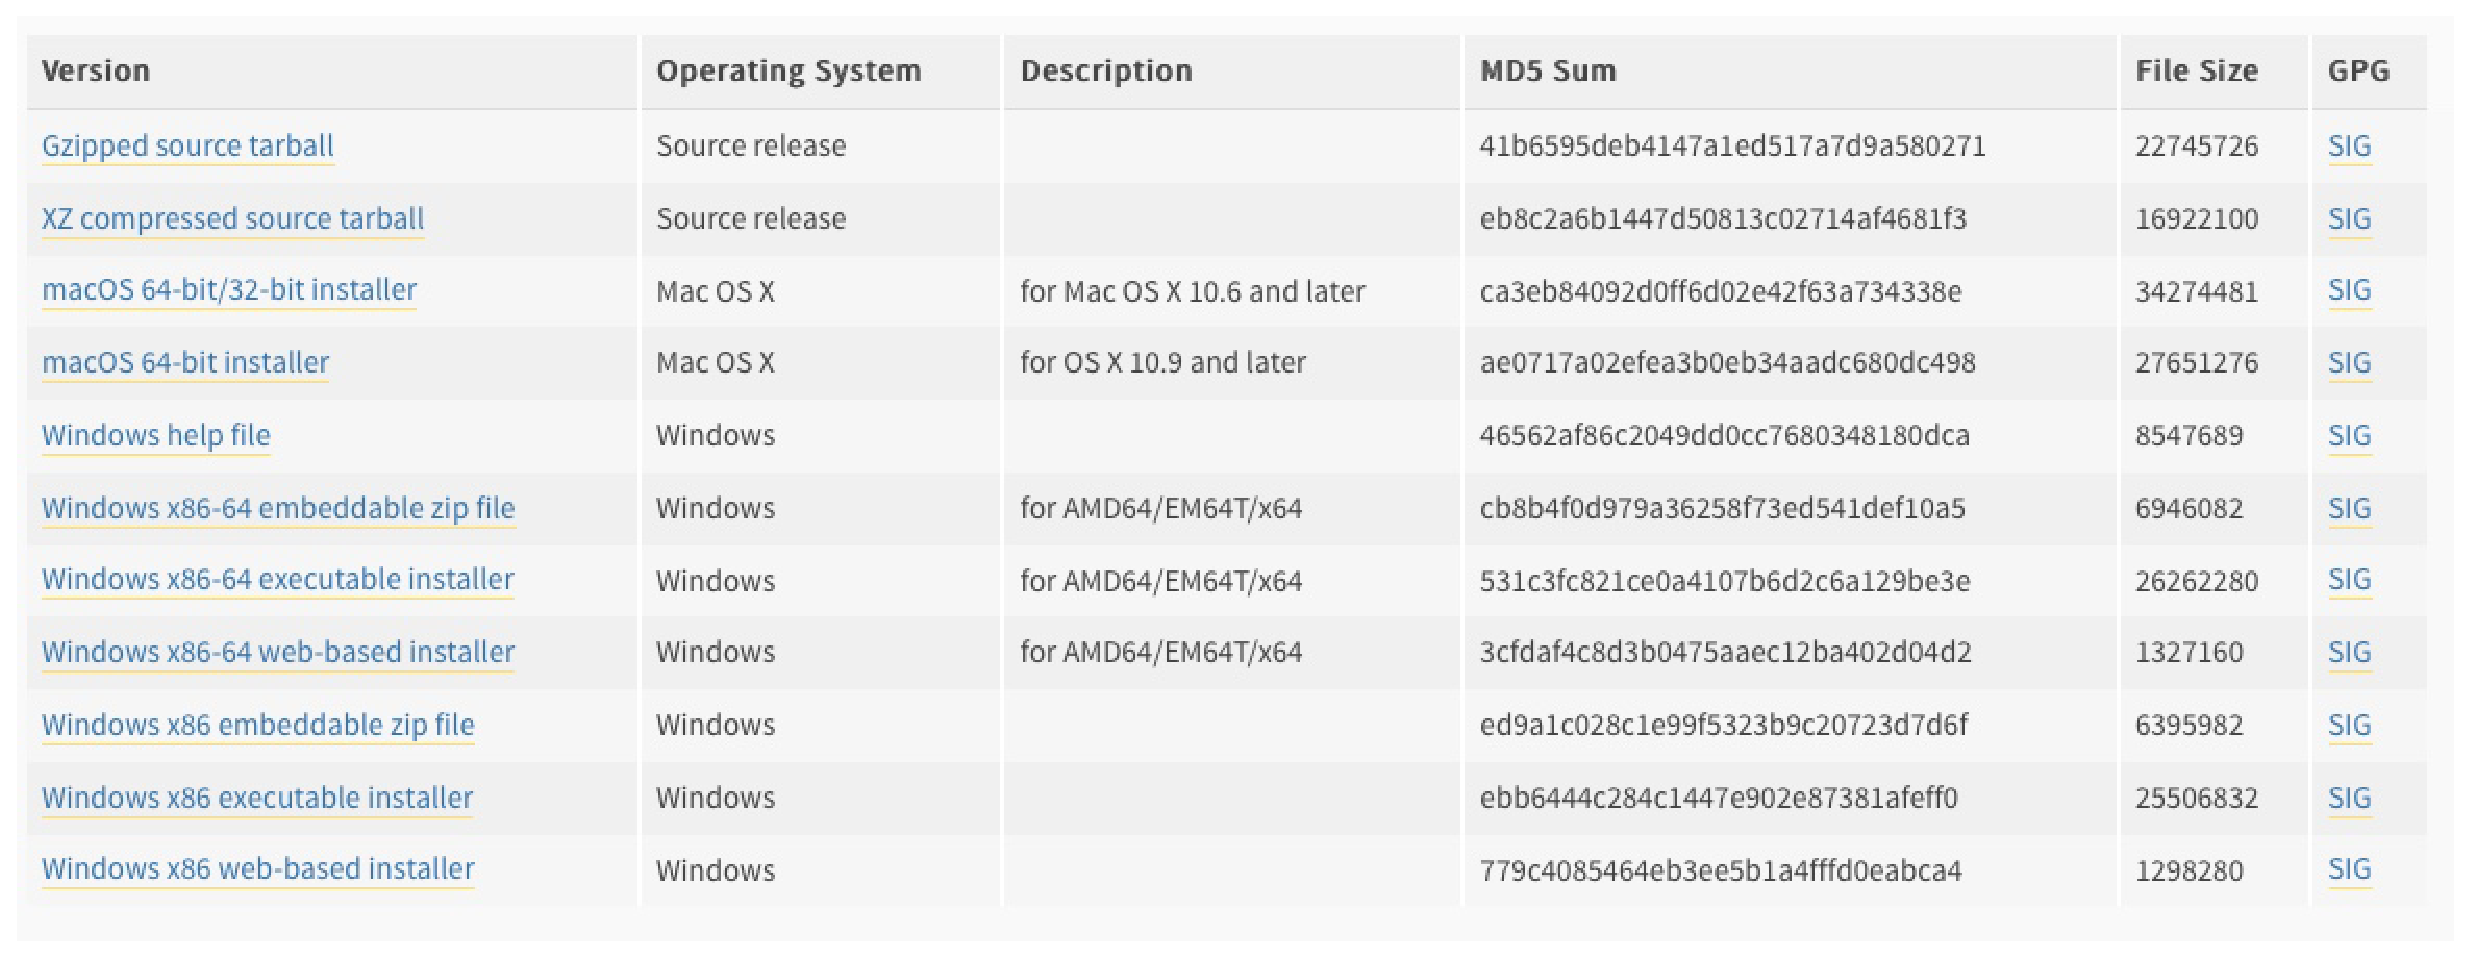
\includegraphics[height=0.38\textwidth]{imagenes/ficheros_inst_windows_mac}
\end{center}
\caption{Ficheros de instalación para Windows y Mac}
\label{fig:instalacion}
\end{figure}

Al terminar la instalación, podremos encontrar en nuestro sistema cuatro herramientas:
\begin{itemize}
	\item Integrated Development and Learning Environment (IDLE). Es un entorno básico de desarrollo de Python. En la sección \ref{sec:eclipsePython} se explica cómo emplear Eclipse como herramienta de desarrollo.
	\item Python 3.7 Module Docs. Documentación de los módulos y paquetes (librerías) de Python instalados en nuestro equipo. En el capítulo \ref{chap:modulosPaquetes} se describe el sistema de módulos y paquetes de Python, y se indica el modo de agregar nuevos paquetes a nuestro sistema.
	\item Python 3.7 Manuals. Documentación muy amplia sobre el lenguaje (tutorial) y sobre otros aspectos relacionados con el funcionamiento de Python en nuestro equipo, como la gestión de módulos/paquetes de nuestra instalación, o la forma de comunicar código desarrollado en C con Python.
	\item Python 3.7. Intérprete de Python. Al ejecutarlo se abre una ventana de comandos con el prompt de Python \texttt{>{}>{}>}, permitiendo un uso interactivo del lenguaje.
\end{itemize}

\begin{figure}
\begin{center}
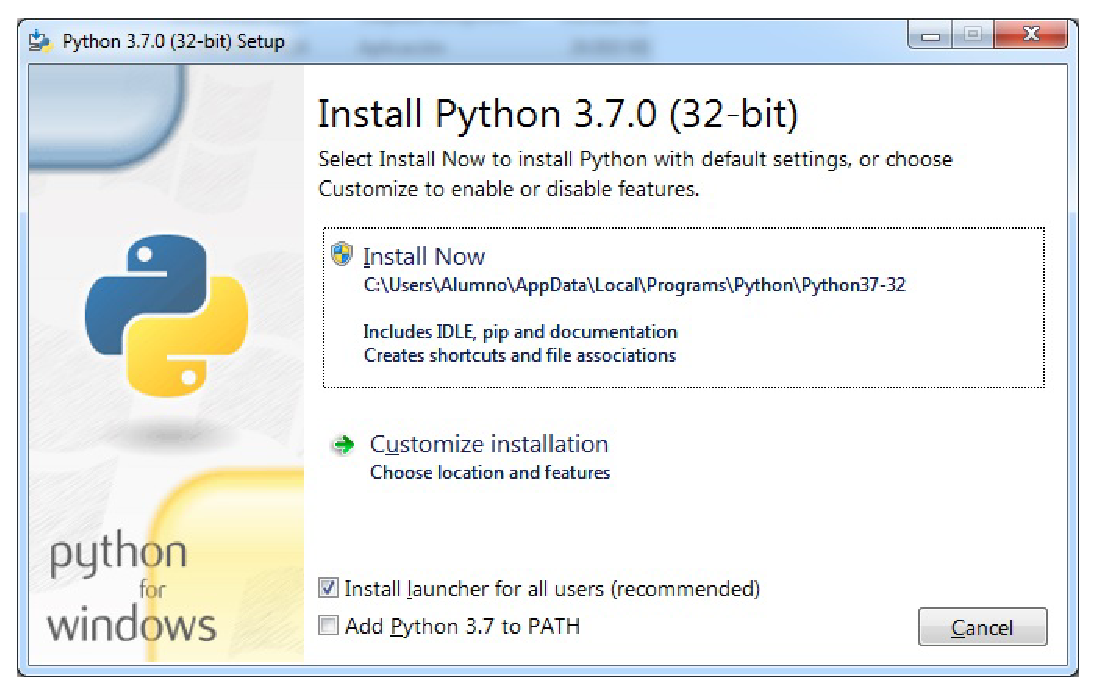
\includegraphics[height=0.5\textwidth]{imagenes/windows}
\end{center}
\caption{Instalación en Windows}
\label{fig:windows}
\end{figure}

\subsubsection{Mac OS X}

Ten en cuenta que un sistema Mac OS X ya tiene alguna versión de Python instalada. Lo más normal es que sea alguna versión de Python 2, como la 2.6 o la 2.7. No pasa nada por tener dos versiones distintas de Python. En la sección \ref{sec:eclipsePython} veremos cómo hay que indicarle al entorno de desarrollo cuál es la que nos interesa usar.

Para este sistema, tenemos dos opciones de instalación de Python 3.7.0 (ver figura \ref{fig:instalacion}): el instalador para Mac OS X 10.9 y versiones posteriores (\emph{macOS 64bit installer}), o el instalador de versiones anteriores del sistema operativo (\emph{macOS 64bit/32bit installer}). Después de la instalación, en el listado de aplicaciones del sistema podremos encontrar una carpeta Python 3.7 que tendrá accesos a:
\begin{itemize}
	\item Integrated Development and Learning Environment (IDLE).
	\item Python Documentation (tutorial del lenguaje, manual de módulos y paquetes, e instrucciones sobre la gestión de los mismos).
	\item Python Launcher. Permite configurar el intérprete que ejecuta los scripts de Python al abrirlos desde Finder.
\end{itemize}

\subsubsection{Linux}

Para instalar Python en Linux, lo más conveniente es usar el comando que gestiona la instalación de paquetes desde un terminal. Por ejemplo, en Ubuntu se haría así:

\begin{lstlisting}
sudo apt-get update
sudo apt-get install python3
sudo apt-get install python3-pip
\end{lstlisting}

Es posible que el comando anterior nos indique que ya tenemos instalada la versión más reciente de Python. Quizás no es la 3.7.0, sino la 3.5.2 o similar. Será suficiente para el desarrollo de las prácticas de la asignatura. La última instrucción instala la herramienta de gestión de paquetes de Python. En caso de usar Fedora, la instalación es muy similar salvo que se debe usar \texttt{yum} en lugar de \texttt{apt-get}.

Con lo anterior, podremos ejecutar desde un terminal el comando \texttt{python3} y se iniciará el intérprete de Python.

\subsection{Eclipse y Python}\label{sec:eclipsePython}

En Autómatas y Lenguajes Formales, vamos a usar Eclipse como entorno de programación de Python. Habitualmente se emplea en la asignatura Programación Orientada a Objetos para el lenguaje Java, de modo que podemos reforzar el manejo de esta herramienta en dos asignaturas. 

Empezamos con la descarga de Eclipse Photon (última versión en el momento de escribir este manual), desde \url{http://www.eclipse.org/photon/}. Al lanzar el instalador de Eclipse, podemos indicar el tipo de entorno que queremos instalar. Las opciones son múltiples, pero ninguna de ellas indica nada sobre Python. Que no cunda el pánico. Se puede instalar una versión para Java (o para C/C++) y luego se modifica para la programación con Python. Recomendamos la primera opción, porque serviría para tener una instalación de Eclipse para las dos asignaturas que emplean este entorno de programación.

Si iniciamos Eclipse después de la instalación, una vez que se indica la ruta al espacio de trabajo (workspace)\footnote{Sería recomendable tener dos espacios de trabajo, uno para Java y otro para Python}, podemos pasar a instalar el plugin que permite emplear Eclipse con Python. Se denomina PyDev, y no hace falta descargarlo e instalarlo independientemente; se puede hacer desde Eclipse, siguiendo estos pasos:

\begin{enumerate}
	\item Entra en el menú \emph{Help}, opción \emph{Install New Software...}
	\item En el campo \emph{Work with:} escribe \texttt{http://www.pydev.org/updates} y pulsa \emph{Enter}.
	\item Marca el paquete \emph{PyDev} y seguidamente pulsa el botón \emph{Next >} dos veces.
	\item Acepta los términos de la licencia del plug-in (Eclipse Public License) y completa la instalación pulsando en \emph{Finish}.
	\item Pulsa en \emph{Restart Now} para que los cambios de Eclipse tengan efecto.
\end{enumerate}

Todavía quedan cosas por hacer. Tenemos que crear un primer proyecto para indicar al plugin PyDev cuál es el intérprete de Python que tiene que usar. Afortunadamente, esto hay que hacerlo sólo al crear el primer proyecto. Seguimos estos pasos:

\begin{enumerate}
	\item En Eclipse, entra en el menú \emph{New} opción \emph{Project}.
	\item Selecciona en el cuadro de diálogo, en la carpeta \emph{PyDev}, el ítem \emph{PyDev Project}. 
	\item Escribe cualquier nombre para el proyecto, como \emph{helloWorld}.
	\item Comprueba que en \emph{Project type} está marcado \emph{Python}. 
	\item En el mismo cuadro de diálogo de creación del proyecto, tendrás que configurar el intérprete de Python que has instalado siguiendo los pasos de la sección anterior. Eso se realiza pulsando donde indica \emph{Please configure an interpreter before proceeding}. 
	\item Selecciona \emph{Advanced Auto-Config} y deja que Eclipse busque las distintas versiones instaladas en el sistema y te permita seleccionar la que quieras usar. Selecciona la versión mayor (\emph{python3.7} o \emph{python3.5} según el sistema). 
	\item A continuación, Eclipse te indicará qué carpetas será necesario añadir al \emph{path} de Python para encontrar los paquetes (librerías) que vas a usar en el código fuente. Pulsa \emph{Ok} al listado por defecto que nos ofrece Eclipse. 
	\item Volviendo al cuadro de diálogo de creación del proyecto, comprueba que en \emph{Grammar Version} aparece seleccionada la opción \emph{Same as interpreter}. 
	\item Pulsa \emph{Finish} para terminar de crear el proyecto. 
\end{enumerate}

Al terminar, veremos que Eclipse muestra dos \emph{perspectivas} para ver el código en iconos arriba a la derecha del entorno de desarrollo: Java y Python. Deberá estar seleccionada esta segunda mientras editemos código Python. La creación de los siguientes proyectos de Python no va a necesitar repetir los pasos para configurar el intérprete de Python, puesto que Eclipse reutilizará esta configuración. Simplemente, bastará con introducir el nombre del proyecto.

\subsubsection{Un paso más en Windows}

Si estás usando Mac OS X o Linux, enhorabuena, ya has terminado con la instalación. Pero si estás con Windows, falta un pequeño detalle que tiene que ver con la codificación usada en ese sistema operativo para los caracteres. Windows emplea un código de caracteres propio, llamado \emph{cp1252}, que no termina de convencer al compilador de Python. Para no tener problemas con los caracteres acentuados, ñ, etc, será mejor que configures el espacio de trabajo de Eclipse para usar \texttt{utf-8} como código de caracteres. Atención: recuerda que te hemos recomendado que crees un espacio de trabajo para Python distinto del que puedas tener para Java. Este cambio podría afectar a tus proyectos Java si estuviesen en el mismo espacio de trabajo que el de Python.

Entra en el menú \emph{Window -> Preferences -> General -> Workspace} y busca al final del cuadro de diálogo \emph{Text file encoding}. Selecciona en \emph{Other} la opción \emph{UTF-8}. Es importante que no edites los ficheros de tus proyectos en Windows con un editor distinto a Eclipse, porque podría estar usando la codificación por defecto de Windows, e intentaría abrir tus ficheros con ella. El lío que se puede montar con los caracteres no ingleses puede ser bastante desagradable.
